\chapter{The Immersed Boundary Method}
\label{immersedBoundaries}
In the following chapter we will study the DG method with immersed boundaries. This chapter is based on \textcite{paper} \\ \indent 
IBMs are characteristic in the way of creating the calculation mesh as they do not rely on body fitted grids but on a level set function $\varphi$ that cuts the cells into the physical and the void region. It therefore makes the mesh generation much easier, as it only needs a cartesian mesh and a function that approximates the level set. Brought along with the cartesian mesh, it is easily parallelisable, thus rendering it convenient for more complex structures that shall be computed on several processors.
	\section{The DG Scheme with Immersed Boundaries}
	We regard an implicit representation of an immersed boundary using the level set function $\varphi$ that parts the calculation area $\Omega_h$ into 
	\todo{align}
	\begin{description}
		\item[the physical region]  $\mathcal{A} = \left\{\vec{x} \in \Omega_h : \varphi (\vec{x}) > 0 \right\}$,
		\item[the void region]  $\mathcal{B} = \left\{ \vec{x}\in \Omega_h : \varphi (\vec{x}) < 0 \right\}$, 
		\item[and the immersed boundary] $\mathcal{I} = \left\{ \vec{x}\in \Omega_h : \varphi (\vec{x}) = 0 \right\}$
	\end{description} 
	as can be seen in  \cref{fig:cutcell}.
	\begin{figure}[htp]
		\centering
		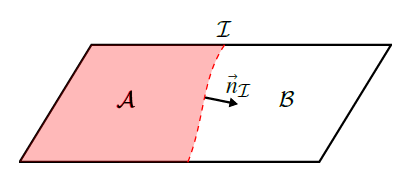
\includegraphics[height=4cm]{ibmcut.PNG}
		\caption{Cut cell with physical (red) and void region (white) \textcite{paper}}\label{fig:cutcell}
	\end{figure}
	In our next step we use the definitions above in \eqref{schwacheFormFlux} considering cell $\mathcal{K}_i$ with the sub-domain $\mathcal{A}_i = \mathcal{K}_i \cap \mathcal{A}$ and the surface $\partial \mathcal{A}_i$. As in cut cells the surface $\partial \mathcal{A}_i$ consists not only of the edges $\left\{\mathcal{E}_{i,e}^\mathcal{A} \right\}_{e = 1, ..., E} = \left\{\mathcal{E}_{i,e} \cap \bar{\mathcal{A}}_i \right\}_{e = 1, ..., E}$ but also of the boundary segment $\mathcal{I}_i = \mathcal{K}_i \cap \mathcal{I}$, the discrete weak formulation using an IBM follows as
	\begin{align}
	\int\limits_{\mathcal{A}_i} \dfrac{\partial c_i}{\partial t}\Phi_{i,j} \, dV +
	\sum_{e=1}^{E_i}\int\limits_{\mathcal{E}_{i,e}^\mathcal{A}} f \left( c^-, c^+, \mathbf{n} \right) \Phi_{i,j} \, dA + \int\limits_{\mathcal{I}_{i}} f \left( c^-, c^+, \mathbf{n}_\mathcal{I} \right) \Phi_{i,j} \, dA - \int\limits_{\mathcal{A}_i} \boldsymbol{f}\left(c_i\right) \cdot \nabla\Phi_{i,j} \, dV = 0
	\label{schwacheFormIBM}
	\end{align}
	with $\mathbf{n}_\mathcal{I} = - \dfrac{\nabla\varphi}{\| \nabla\varphi \|}$.
	In intersected cells the mass matrix is defined by
	\begin{align}
		(\mathbf{M_i})_{k,j} := \int\limits_{\mathcal{A}_i}\Phi_{i,k}\Phi_{i,j}\, dV
	\end{align}
	and the discrete operator by
	\begin{align}
		(\mathbf{f}_i)_j := \sum_{e=1}^{E_i}\int\limits_{\mathcal{E}_{i,e}^\mathcal{A}} f \left( c^-, c^+, \mathbf{n} \right) \Phi_{i,j} \, dA + \int\limits_{\mathcal{I}_{i}} f \left( c^-, c^+, \mathbf{n}_\mathcal{I} \right) \Phi_{i,j} \, dA - \int\limits_{\mathcal{A}_i} \boldsymbol{f}\left(c_i\right) \cdot \nabla\Phi_{i,j} \, dV.
	\end{align}
	The difficulty of the IBM lies in the correct evaluation of $\mathcal{A}_i$ and $\mathcal{I}_i$ and in the agglomeration of intersected cells with very small volume fractions 
	\begin{align}
		\text{frac}(\mathcal{A}_i) = \dfrac{\text{meas}(\mathcal{A}_i)}{\text{meas}(\mathcal{K}_i)}
	\end{align} 
	as we will discuss in section \cref{cellAgglomeration}.
	
	\section{RK Time Discretisation with Immersed Boundaries}
	In this thesis we only use explicit Euler time discretisation for immersed boundary problems as we are only interested in the steady state:
	\begin{align}
		\mathbf{c_i}(t_1) = \mathbf{c_i}(t_0)-\Delta t \mathbf{M}_i^{-1} \mathbf{f}_i (c).
	\end{align}
	Using IBMs we have to modify the stability criterion and therefore use the modified step restriction
	\begin{align}
		\Delta t \leq \dfrac{c_{CFL}}{2P+1} \dfrac{\sqrt[D]{\text{meas}(\mathcal{A}_i)}}{\|\mathbf{u} \| + a}
		\label{timestepIBM}
	\end{align}
	which is strongly influenced by the sub-cell $\mathcal{A}_i$ with the smallest volume.
	
	\section{Cell Agglomeration}
	\label{cellAgglomeration}
	As can be seen in \eqref{timestepIBM} the time step size is strongly restricted in cells with very small volume fractions. This leads to an elongated calculation process thus rendering the method impractical. Therefore we need to agglomerate those small cells to larger ones using a cell agglomeration factor $0 \leq \alpha \leq 1$. \\
	The cell agglomeration strategy depends on finding the source cells $\left\{\mathcal{K}_s^\text{src} \right\}_{s=1,...,S}$ with $\text{frac}(\mathcal{A}_i) \leq \alpha$ and agglomerating them to the neighbouring cell with the highest volume fraction, namely target cell $\mathcal{K}_s^\text{tar}$. In \cref{fig:agglomeration} you can see the cell agglomeration for a smaller (b) and a bigger (c) agglomeration factor. \\
	\begin{figure}[htp]
		\centering
		\begin{minipage}[b]{0.3\textwidth}
			\centering
			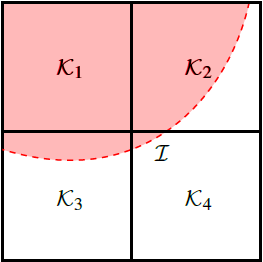
\includegraphics[height=4.5cm]{ibminitmesh.PNG}
			\caption*{(a) Initial mesh partitioning \newline \newline}
			\label{fig:init}
		\end{minipage}%
		\begin{minipage}[b]{0.3\textwidth}
			\centering
			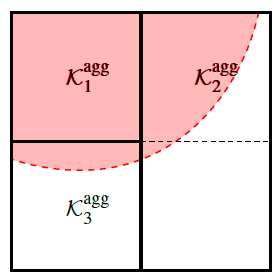
\includegraphics[height=4.5cm]{ibmagglomklein.PNG}
			\caption*{(b) Cell agglomeration with small agglomeration threshold}
			\label{fig:agglomgklein}
		\end{minipage}
		\begin{minipage}[b]{0.3\textwidth}
			\centering
			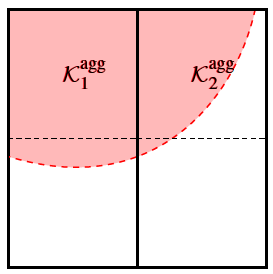
\includegraphics[height=4.5cm]{ibmagglomgross.PNG}
			\caption*{(c) Cell agglomeration with bigger agglomeration threshold}
			\label{fig:agglomgross}
		\end{minipage}%
		\caption{Cell agglomeration, taken from \cite{paper}}\label{fig:agglomeration}
	\end{figure}
	
	For the neighboring cells are weakly coupled via fluxes, the basis $\vec{\Phi}_i$ can be extended from the target cell into the source cell. Therefore the source cell can formally be deleted from the discretisation mesh, reducing it to $\left\{\mathcal{K}_s^\text{agg} \right\}_{i=1,...,N-S}$.
	As can be found in \textcite{paper}, it however does not reflect the actual implementation in \gls{bosss} which only requires few cell-local matrix-vector products per time-step, thus not affecting the parallel efficiency.
	
	\section{Simulation Parameters Concerning Stability and Runtime in \glsentrytext{bosss}}
	\label{parameters}
	
	In the following we will describe some of the preferences for the \gls{cns} solver that can be modified in order to stabilise the computations. 
	
	\paragraph{LevelSetQuadratureOrder}
	The first preference is the \textit{LevelSetQuadratureOrder}. It describes the quadrature order that is used for the evaluation of volume and edge operators. It is set to an integer; we will use a constant
	\begin{lstlisting}
		c.LevelSetQuadratureOrder = 8;
	\end{lstlisting}
	in \cref{eulerVerification} as it is important to have comparable results for the verification and a degree dependent order
	\begin{lstlisting}
		c.LevelSetQuadratureOrder = 3*dgDegree;
	\end{lstlisting}
	in \cref{viscousCylinder} as it is more important to produce efficient and fast though stable results. 
	
	\paragraph{SIPGPenaltyConstant}
	 The second preference that we used is the \textit{SIPGPenaltyConstant}. It is set to a double that should be greater than one and describes the weighting of the viscous terms. For the stability of the computation it is essential that the numerical flux functions that are used for the discretisation of the viscous terms are consistent. This can be achieved by different methods; one of those being the \gls{sipg} which we are using which introduces the penalty factor. In \cref{viscousCylinder} we will set 
	 \begin{lstlisting}
		c.SIPGPenaltyConstant = 5.0;
	 \end{lstlisting}
	for our calculations.
		 
	\paragraph{NodeCountSafetyFactor}
	The last factor that we will vary for a better stability is the \textit{NodeCountSafetyFactor}. This factor, that is also set to a double, indicates the number of the nodes with respect to the number of modes that will be used during the quadrature. By standard \gls{bosss} sets it to $1.0$; in our calculations we mostly used a NodeCountSafetyFactor of $2.0$  in \cref{eulerVerification} and of $5.0$ in \cref{viscousCylinder} though it has been modified for few calculations in order to get them more stable.\\\\
	
     All of these factors should be set just high enough in order to ensure a accurate and stable solution and the shortest possible runtime at the same time. 
     

	